\documentclass[notes]{beamer}
\usepackage{graphics}
\usepackage{url}
\usepackage {amssymb}
\usepackage{xcolor}
\usepackage{tikz}
\usetikzlibrary{positioning}
\usetikzlibrary{shadows}
\usetikzlibrary{arrows,automata,shapes,calc}
%\usepackage{enumitem}
%\usepackage{onimage}
 \usepackage{standalone}

\usecolortheme{crane}
\parskip=10pt plus 1pt


\begin{document}
  \title{Ricardo, Rent, and Roemer: \\Class and exploitation in the financialized city}

%\author[Dr. David Robinson,Kirsten Wright]{Dr. David Robinson\inst{Laurentian University}  \and Kirsten Wright\inst{University of Waterloo} }

\author{Dr. David Robinson\hspace{30pt}Kirsten Wright\\
           Laurentian University, University of Waterloo}%\\
%             \ \\
%           \small Prepared for the Annual Conference of the \\
%           \small  Canadian Economic Association, June 3-5, 2021}
 
\def\defn#1{{\color{red} #1}}

 %\logo\pgfdeclareimage[height=0.5cm]{INORDlogo\_April2012-eps-converted-to.pdf}{tu-logo}


%% 
%\usepackage{graphicx}
%% \usepackage[table]{xcolor}
%
%\begin{document}
\begin{frame}
\titlepage
\end{frame}
%%%%%%%%%%%%%%%%%%%%%%%%%%%%%%%%%%%%%%%%%%%%%%%%%%%% FRAME

\begin{frame}\frametitle{Outline}
\tableofcontents
\end{frame}


\section{A Question}%%%%%%%%%%%%%%%%%%%%%%%%%%% FRAME

\begin{frame}\frametitle{}

\begin{itemize}
\item Housing prices keep going up
\item Young people can't buy houses.\vspace{.5cm}

\hspace{2cm} {\Large Its just a bubble? } \vspace{.5cm}\pause

\item The global population is moving to cities

\item technological change is accelerating
\item the global wealth  distribution is getting worse

\end{itemize}\vspace{.5cm}

\hspace{2cm}{\Large Are all these economic features }

\hspace{2cm} {\Large of our modern world related?}\vspace{.5cm}\pause

\hspace{6cm}We think so.

\end{frame}
\section{The Model and it's History} %%%%%%%%%%%%%%%%%%%%%%%%%%%%%%%%%%%%%% FRAME
\begin{frame}\frametitle{A note:}
This is a tricky paper to present. We have been expecting an audience with distinguished economists, green activists, undergraduate economics students, and possibly academics from other fields,  and even some Marxists-at-large.

It is a fairly technical paper using a lot of tricks of the trade, and we will play that part down so we can focus on the story

We are combining ideas about the source of income for various classes from Ricardo, and Marx with a modern growth models and and standard urban model. %He  focussed on the exploitation of the  rising class of industrial workers, but his thinking, unlike Ricardo's, was  much more dynamic.
\end{frame}
%%%%%%%%%%%%%%%%%%%%%%%%%%%%%%%%%%%%%%%%%%%%%%%%%%% FRAME
\begin{frame}\frametitle{The model}
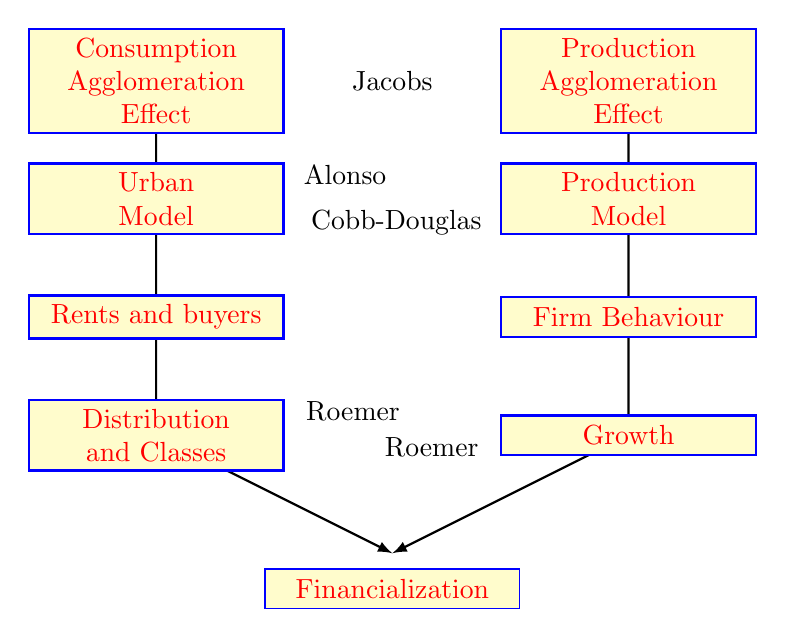
\begin{tikzpicture}[scale=.5]
%\tikzset{every node/.style={red, draw=blue, fill=yellow!20, minimum size=0.5cm, text width =3cm, align = center},}	
\def \left {6}
\def \right {-\left}
\def \top {10}
\def \skip {-3}
\node at (0,\top) {Jacobs};
\node at (-1.2,{\top+.8*\skip}) {Alonso};
\node at (0.1,{\top+1.2*\skip}) {Cobb-Douglas};
\node at (-1,{\top+2.8*\skip}) {Roemer};
\node at (1,{\top+3.1*\skip}) {Roemer};
%\node at (0,{\top+4.3*\skip}){Financialization};

\tikzset{every node/.style={red, draw=blue, fill=yellow!20, minimum size=0.5cm, text width =3cm, align = center},}	
\draw[-latex,  thick, to path={-| (\tikztotarget)}, outer sep=2pt](\left,\top)node {Production \\ Agglomeration\\ Effect} -- ( \left,{\top+\skip})node {Production \\ Model}--( \left,{\top+2*\skip})node {Firm Behaviour} -- ( \left,{\top+3*\skip})node{Growth}-- (0,{\top+4*\skip} ); 

\draw[-latex,  thick, to path={-| (\tikztotarget)}](\right,\top)node {Consumption \\ Agglomeration\\ Effect} --( \right,{\top+\skip})node {Urban \\ Model}--( \right,{\top+2*\skip})node {Rents and buyers} -- ( \right,{\top+3*\skip})node{Distribution and Classes}-- (0,{\top+4*\skip} ); 
\node at (0,{\top+4.3*\skip}){Financialization};

\end{tikzpicture}
\end{frame}

%%%%%%%%%%%%%%%%%%%%%%%%%%%%%%%%%%%%%%%%%%%%%%%%%%%% FRAME
%\begin{frame}\frametitle{}
%
%
%%The point here is that Marx identified the dominant economic transformation of his time and produced a theory of how it evolved in historical time.  Marx took over Hegel's teleological account of history and developed a materialist theory ( I would call it an \textbf{economic} theory) of historical development class relations and distribution.
%
%Neither Marx nor Ricardo were particularly good at calculus, and they didn't have the tools of modern economics, so they did not talk about classes the way a modern economist would. On the other hand, and most economists are not very good at history and especially class issues, so the modern framework has not been applied to the recent transformation of the economic base.
%
%That's what this paper is trying to do. 
%
%
%\end{frame}
%%%%%%%%%%%%%%%%%%%%%%%%%%%%%%%%%%%%%%%%%%%%%%%%%%%% FRAME
\begin{frame}\frametitle{Production, rent, surplus labour, and exploitation}%A run through the history of economic thought to collect some tools}
% These are the big names in classical rent theory
\begin{itemize}
\item Ricardo of had two factors of production: land and labour. 
\textbf{\textit {The class that owned all the land earned land rents: exploited the peasants labour.}}

\item  In the industrial revolution, which Marx focussed on, English landowners replaced peasants with sheep creating a pool of ``free labour'' that was cheap. %Das Kapital. Kritik der politischen Ökonomie,  1867–1883)

\textbf{\textit {The class that owned all the produced capital needed for industrial production earned land rents - (Marx called it surplus value): exploited the free labour.}}

\item After Marx, Henry George, identified something like Ricardian land rents as the basis of exploitation.
%\begin{quotation}{\tiny \noindent by far ``the most famous American economic writer'' and ``author of a book which probably had a larger world-wide circulation than any other work on economics ever written''}
%\end{quotation}
\item Roemer analyzed class and exploitation in a multi-factor GE economy. 
\end {itemize}
\end{frame}

%%%%%%%%%%%%%%%%%%%%%%%%%%%%%%%%%%%%%%%%%%%%%%%%%%%% FRAME
\begin{frame}\frametitle{}

\begin{itemize}  
\item After Ricardo, Marx, and George, more mathematical economists described production with  ``Functions'', such such as the Cobb-Douglas  form (1927)
\begin{eqnarray*}
Y=& f(Land, Labour, Capital) \\ 
Y=&L^0 K^{\textcolor{red}{\alpha}} N^{\textcolor{red}{\beta}}
\end{eqnarray*}


\item The values of $\alpha$ and $\beta$. are very important. 

If $\alpha+\beta >1$ a single firm takes over the world.  

If $\alpha+\beta <1$ a large city has competitive firms and, as Marshall pointed out, zero profits in equilibrium*.

\pause

% Marx and Ricardo would have understood this - they both grasped diminishing marginal returns, but the techniques had not been developed   (Qualifications: Von Thunen, The Isolated State (1826)  Cournot   Researches on the Mathematical Principles of the Theory of Wealth (1838)  

\item \textbf{\color{red}Technical Discovery:} production was increasing more rapidly than the combined supply of land labour and capital predicted. 

\item Solow introduced a term, $A(t)$,  called ``total factor productivity.'' 

\[Y= \textcolor{red} {A(t)} L^0 K^\alpha N^\beta\]

\end {itemize}
\end{frame}

%%%%%%%%%%%%%%%%%%%%%%%%%%%%%%%%%%%%%%%%%%%%%%%%%%%% FRAME
\begin{frame}\frametitle{}
\begin{itemize} 


\item In the 1960's  growth economists fiddled with this idea calling it things like ``labour augmenting technological change,'' ``human capital,'' ``learning,'' ``technology,''

\item They realized that human skills, knowledge, institutions,  and social organization  
are factors of production like labour, land and capital.  \vspace{1cm}

In Endogenous Growth theories, ``$A$'' depends on education spending, investment in invention, investment in previous production. 

These are things that can be influenced by government policy.



\end {itemize}
\end{frame}

%%%%%%%%%%%%%%%%%%%%%%%%%%%%%%%%%%%%%%%%%%%%%%%%%%%% FRAME
\begin{frame}\frametitle{The city as the source of productivity}
\begin{itemize}

\item In 1985 Jane Jacobs published \textbf{Cities and the Wealth of Nations}, arguing that urban agglomeration itself accounted for a great deal of the increase in productivity that mystified the growth theorists. In $N$ is urban population,

\[Y=  \textcolor{red} {A(N)}K_i^\alpha N_i^\beta\]

\item The difference between total labour $N$ and the labour used by an individual firm  $N_i$  matters. The firm can't take credit for increasing productivity. It is a social product.

\item \textbf{This raises the question, ``Who should get that benefit?''}
%\item In 1990 John Porter kicked off a project that led to cluster theory and a a focus on  agglomeration economies.

\end {itemize}

\end{frame}


\section{The Urban Model}%%%%%%%%%%%%%%%%%%%%%%%%%%%%%%%%%%%%%%%%%% FRAME
% \begin{frame}\frametitle
{A parallel development of rent theory}
\begin{itemize} 

\item In 1964, William Alonso published \textbf{Location and Land Use}, in which he defined a model %of the formation of land rent in urban environments. He 
that specifically linked urban agglomeration to land rents and this became the central model in modern urban economics.

\item We use an \textbf{Alonso-Jacobs model} to explore the distribution surplus value.
\end {itemize}
% \end{frame}

%%%%%%%%%%%%%%%%%%%%%%%%%%%%%%%%%%%%%%%%%%%%%%%%%%%% FRAME
\begin{frame}\frametitle{Alonso's Circular City}
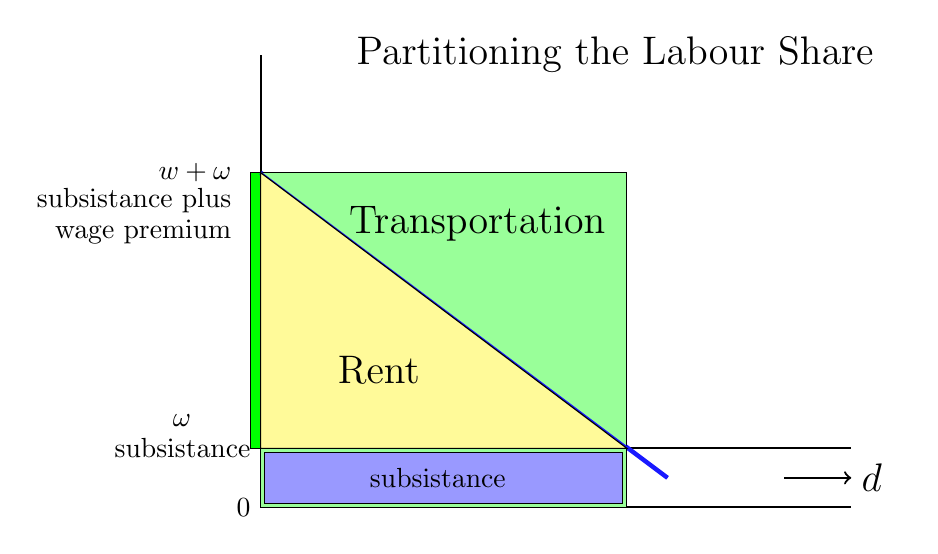
\begin{tikzpicture}[scale=.5]
\def\bndmax{5}        %https://tex.stackexchange.com/questions/68462/filling-a-complex-region-with-tikz
\def\bndmin{0.2}
\def \n {10}  % height of y axis
\def \d {15}  % length  of x axis
\def \t {.75}  %  cost of transportation per unit x
\def \th {1}   %
\def \w {7}    %  wage premium
\def \om{1.5}%  omega =rural wage Zero for urban population
\def \azero{2}
\def \aprime {-.0}	
\tikzset{func/.style={thick,color=blue!90}}	

% FIRST FIGURE just axes
\draw [thick] (0,-\om) --(\d,-\om);  			% Zero for rural population
\draw [thick] (0,-\om)node[left]{$0$} --(0,\n);	% Y axis
%\node at (0,\n+0.5){\large$Rent$};

\draw [thick] (0,0)node[left]{subsistance}--(\d,0);
\node a t(-2,.7) {$\omega$};
\node[left=.25] at (0,\w){$w+\omega$};
\node[left=.25] at (0,\w-.7){subsistance plus};
\node[left=.25] at (0,\w-1.5){wage premium};	

%\foreach \xi in {0,..., \n} \draw (\xi,0)--(\xi,-.1)node[below=1]{\small$\xi$};
%\foreach \yi in {1,...,\n} \draw (0,\yi)--(-.1,\yi)node[left]{$\yi$};
%\foreach \i in {1,4,9,16} {
\node at (7,-\om/2){people scattered uniformly across the land  };

%SECOND FIGURE WITH AGGLOMERATION WAGE
\pause %  add urban production and net wage
\draw[fill=white, white] (0.1,-0.1) rectangle (14,-\om+.1);
\draw [fill=green] (-.25, 0) rectangle(.25, \w);
\node[right] at  (.25, \w/2){Added Productivity};
\node[right, text width = 3cm] at  (10,9){Where does the increase in productivity come from?};
\draw [ thick, ->](13.3,-\om/2)--(15, -\om/2)node [right] {\Large $d$};

%  THIRD FIGURE  add wage profile
\pause
\node[right, white, fill=white,  text width = 3cm] at  (10,9){Where does the increase in productivity come from?};
\draw[func, domain=0:\w/\t+1,ultra thick] plot [samples=200] (\x,{\w-\t*\x}); %Net wageprofile  for 
\node[right, white, fill=white] at  (.25, \w/2){Added Productivity};
\node[right, fill=white, text width =3.5cm ] at  (1, \w/2){Declining wage  net \\of transportation\\ costs $T(d)$ };

%   FOURTH FIGURE     commuters
\pause
\draw[fill=blue!40] (0.1,-0.1) rectangle (9.2,-\om+.1);
\node at (4.5,-\om/2){commuters};

%   FOURTH FIGURE    wage bill
\pause %add total new value
\draw[fill=green!40] (0,-\om) rectangle(9.30,\w);% new product
\node at (4.5,\w/2){\Large urban wage bill};

%%   FIFTH FIGURE   distribution
\pause
\node at (9,\n){\Large Partitioning the Labour Share};

\draw[fill=green!40] (0,-\om) rectangle (9.30,\w);% new product repeat
\draw[func, domain=0:\w/\t+1] plot [samples=200] (\x,{\w-\t*\x}); %rent profile
\draw[fill=blue!40] (0.1,-0.1) rectangle (9.2,-\om+.1);
\node at (4.5,-\om/2){subsistance};
\draw[fill=yellow!40] (0.,0.) -- (0,7)--(9.30,0.)--cycle;% Rent \w-.2
\node at (3.,2){\Large Rent}; 		%Rent 
\node at (5.5,5.7){\Large Transportation};
 \end{tikzpicture}
\end{frame}

\section{Distributional issues}%%%%%%%%%%%%%%%%%%%%%%%%%%%%%%%%%%%%%%%%%% FRAME
\begin{frame}\frametitle{Who gets the rent?}

\begin{itemize}
\item It is capitalized into land values - 
\item The original land owners get the increase in land value. Why should they?
\item They realize the value if they sell the property.
\item New owners MAY get rents from future productivity increases.\vspace{1cm}
\end {itemize}
\end{frame}
%%%%%%%%%%%%%%%%%%%%%%%%%%%%%%%%%%%%%%%%%%%%%%%%%%%% FRAME
\begin{frame}\frametitle{Two notes}

\begin{itemize}
\item Property taxes take some of the value for the community. How much is the community entitled to?

\item In 1977, Joseph Stiglitz  proved the "Henry George Theorem" that said urban land rents would be all you needed to pay for public goods that make a city attractive. 

\item A 100\% tax on capital gains in land is the logical consequence
% My note on this is cited in the wikipedia article on the Henry George Theorem!
\end {itemize}


\end{frame}

%%%%%%%%%%%%%%%%%%%%%%%%%%%%%%%%%%%%%%%%%%%%%%%%%%%% FRAME
\begin{frame}\frametitle{Class Analysis: The city so far.}
\begin{itemize}
\item Before  anyone sells their property there are two classes: Capitalists and workers.
\item when a property owner sells the property they  own capital, which mean s they receive an income share of future wages: They are members of an intermediate class of small capitalists.
\item They may invest and continue working or work less and live in part off of the labour of others.  
\item John Roemer in \textbf{A General Theory of Exploitation and Class} (1982) offers  formal definitions of `exploited' and `exploiter'. This group falls in both  categories and can be classified as neither

\end {itemize}

\end{frame}
\section{Consumption Amenities} %%%%%%%%%%%%%%%%%%%%%%%%%%%%%%%%%%%%%%% FRAME
\begin{frame}\frametitle{Adding consumption amenities}
There can be agglomeration benefits of urban life - $ \textcolor{red}{\mathcal{A}(N,d)}$
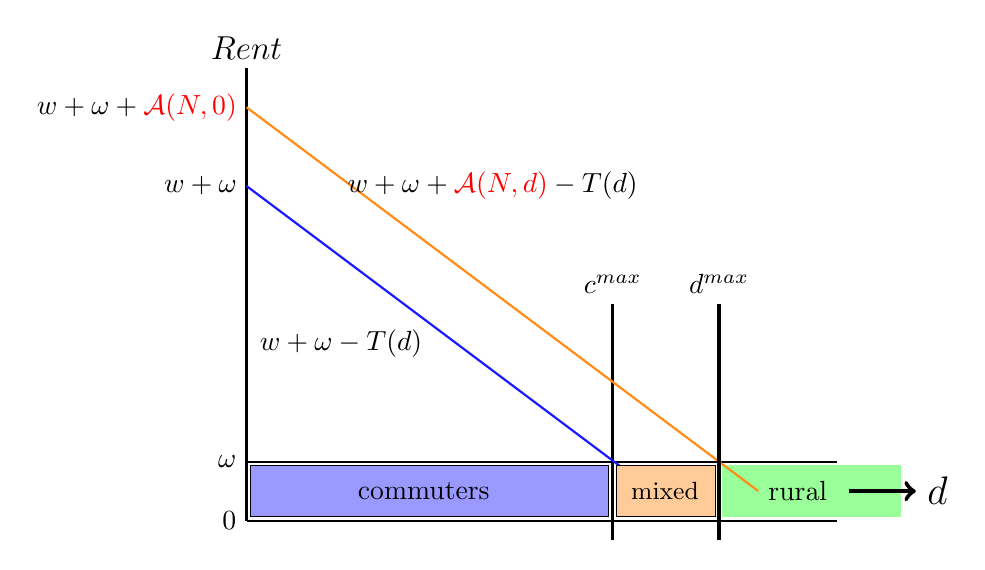
\begin{tikzpicture}[scale=.5]
\def\bndmax{5}        %https://tex.stackexchange.com/questions/68462/filling-a-complex-region-with-tikz
\def\bndmin{0.2}
\def \n {10}  % height of y axis
\def \d {15}  % length  of x axis
\def \t {.75}  %  cost of transportation per unit x
\def \th {1}   %
\def \w {7}    %  wage premium
\def \om{1.5}%  omega =rural wage Zero for urban population
\def \azero{2}
\def \aprime {-.0}	
\tikzset{func/.style={thick,color=blue!90}}	

\draw [thick] (0,-\om) --(\d,-\om);  	% Zero for rural population
\draw [thick] (0,-\om)node[left]{$0$} --(0,\n);			% Zero for urban population
\node at (0,\n+0.5){\large$Rent$};

\draw [thick] (0,0)node[left]{$\omega$}--(\d,0);
\node[] at ({\d+.5},-\om/2) {\Large $d$};
%\foreach \xi in {0,..., \m} \draw (\xi,0)--(\xi,-.1)node[below=1]{\small$\xi$};
%\foreach \yi in {1,...,\n} \draw (0,\yi)--(-.1,\yi)node[left]{$\yi$};
%%\foreach \i in {1,4,9,16} {


\draw [very thick](9.3,-2)-- ++ (0,6)node[above]{$c^{max}$};;

% solid color for commuters
\draw[fill=blue!40] (0.1,-0.1) rectangle (9.2,-\om+.1);
% Net wageprofile  for commuters
\draw[func,domain=0:\w/\t+1] plot [samples=200] (\x,{\w-\t*\x});
	%	\draw[func,domain=0:\m, dashed] plot [samples=200] (\x,{\w+\azero-\th*\x+\aprime*\x});
\node[left] at (0,\w){$w+\omega$};	
\node at (2.4,3.){$w+\omega-T(d)$};
\node at (4.5,-\om/2){commuters};

% solid color for transition
\draw[fill=orange!40] (9.4,-0.1) rectangle (11.9,-\om+0.1);
	\node[text width=2] at (9.84,-\om/2){\small mixed};
\draw[fill=green!40, green!40] (12.1,-0.1) rectangle (16.6,-\om+0.1);
\node at (14,-\om/2){rural};
\draw [ ultra thick, ->](15.3,-\om/2)--(17, -\om/2)node [right] {\Large $d$};
% Net amenity profile  for commuters
	\tikzset{func/.style={thick,color=orange!90}}	
		\draw[func,domain=0:\d-2] plot [samples=200] (\x,{\w+\azero-\t*\x+\aprime*\x});
	\node[left] at (0,{\w+\azero} ){$w+\omega + \textcolor{red}{\mathcal{A}(N,0)}$};
	\node at (6.25,7 ){$w+\omega +\textcolor{red}{\mathcal{A}(N,d)}-T(d)$};

	\draw [very thick](12,-2)-- ++ (0,6)node[above]{$d^{max}$};
 
 \end{tikzpicture}
% ****   notice mixed: they get benefits don't work and pay rent. ***Rent is higher!!
\end{frame}

%%%%%%%%%%%%%%%%%%%%%%%%%%%%%%%%%%%%%%%%%%%%%%%%%%%% FRAME
\begin{frame}\frametitle{Who gets the amenities?}
\begin{itemize}
\item They go to property owners 

\item When owners sell they capture the capitalized  value of the amenity

\item Tenants pay rent that captures the value of the amenity for the land owner. 


\end{itemize}



\end{frame}


\section{The evolution of the Urban System}%%%%%%%%%%%%%%%%%%%%%%%%%%%%%%%%%%%%%%%% FRAME
\begin{frame}\frametitle{Growth andPrices }

\begin{itemize}
\item If wages do not rise, the new owners do not get any of the captalized value of the rent

\item  Will the urban wage premium rise? 
	\begin{quotation}
	In our model, capital captures some of the agglomeration benefits in production. It earns an excess return or super-profit. This attracts more capital, which demands more labour. This pushes up the wage to attract more workers. 
	\end{quotation}
	
\item More labour increases agglomeration effect, resulting in more investment and  more growth. 
\item capital will compete for the \textbf{perpetual capital gain from urban  land} 


\pause
\item Therefore \textcolor{red}{land prices rise as long as there is a  supply of workers}
\end{itemize}


\end{frame}
%%%%%%%%%%%%%%%%%%%%%%%%%%%%%%%%%%%%%%%%%%%%%%%%%%%% FRAME
\begin{frame}\frametitle{Urban land becomes a \textbf{speculative asset} }
So who buys speculative assets?
 \pause
 
\begin{itemize}
\item {\Large Returns on capital are higher for wealthy investors}
\item Why? People with higher wealth get 
	\begin{enumerate}
	\item lower borrowing costs
	\item higher borrowing limits,  allowing more leverage
	\item professional investment advice
	\end{enumerate}
\item People with higher wealth may be less risk-averse 
\item People with higher wealth are generally more liquid 
\item People with higher wealth may have more confidence about long term investments
\end{itemize}

\Large The wealthy will bid more than the less wealthy.

\tiny This contradicts a standard assumption in modelling


\end{frame}


%%%%%%%%%%%%%%%%%%%%%%%%%%%%%%%%%%%%%%%%%%%%%%%%%%% FRAME
\begin{frame}\frametitle{Who will the new owners be?}


\begin{enumerate}
\item  land prices rise continually
\item urban land becomes a speculative asset
\item Ownership of urban land is increasingly concentrated in the wealth holding class as a financial asset 
\item new workers are shut out of the land market.
\end{enumerate}



\end{frame}
%%%%%%%%%%%%%%%%%%%%%%%%%%%%%%%%%%%%%%%%%%%%%%%%%%% FRAME

\begin{frame}\frametitle{Conclusions}
\begin{enumerate}
\item attempts to make home ownership for new entrants affordable can only bid up prices 
\item The fundamental problem is private ownership of land, which allows individuals and capital to capture the social surplus value generated by agglomeration.
\end{enumerate}



\end{frame}

%%%%%%%%%%%%%%%%%%%%%%%%%%%%%%%%%%%%%%%%%%%%%%%%%%%%% FRAME
\begin{frame}\frametitle{}
%\includegraphics[scale=1]{x.jpg}

\end{frame}

\end{document}


%%%%%%%%%%%%%%%%%%%%%%%%%%%%%%%%%%%%%%%%%%%%%%%%%%%% FRAME
\begin{frame}\frametitle{}
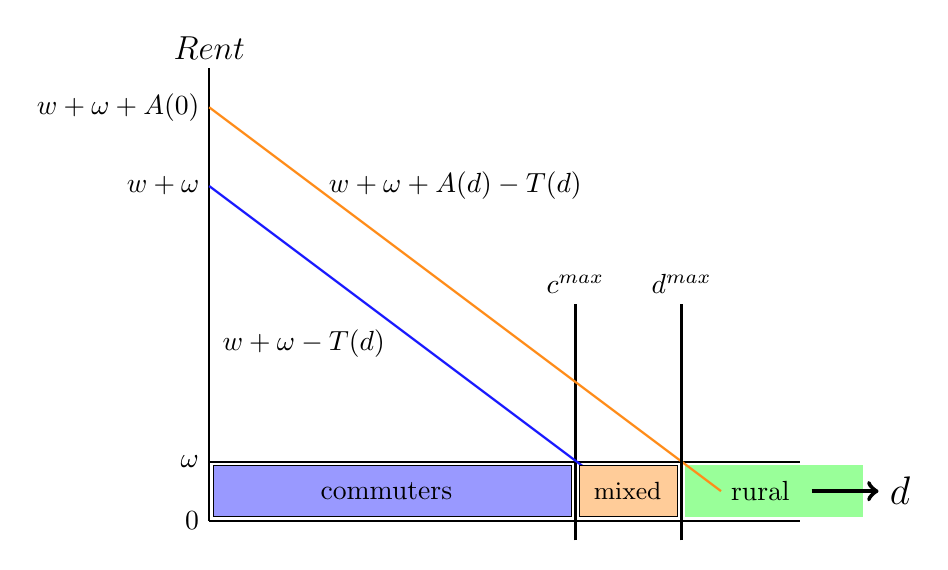
\begin{tikzpicture}[scale=.5]
\def\bndmax{5}        %https://tex.stackexchange.com/questions/68462/filling-a-complex-region-with-tikz
\def\bndmin{0.2}
\def \n {10}  % height of y axis
\def \d {15}  % length  of x axis
\def \t {.75}  %  cost of transportation per unit x
\def \th {1}   %
\def \w {7}    %  wage premium
\def \om{1.5}%  omega =rural wage Zero for urban population
\def \azero{2}
\def \aprime {-.0}	
\tikzset{func/.style={thick,color=blue!90}}	

\draw [thick] (0,-\om) --(\d,-\om);  	% Zero for rural population
\draw [thick] (0,-\om)node[left]{$0$} --(0,\n);			% Zero for urban population
\node at (0,\n+0.5){\large$Rent$};

\draw [thick] (0,0)node[left]{$\omega$}--(\d,0);
\node[] at ({\d+.5},-\om/2) {\Large $d$};
%\foreach \xi in {0,..., \m} \draw (\xi,0)--(\xi,-.1)node[below=1]{\small$\xi$};
%\foreach \yi in {1,...,\n} \draw (0,\yi)--(-.1,\yi)node[left]{$\yi$};
%%\foreach \i in {1,4,9,16} {


\draw [very thick](9.3,-2)-- ++ (0,6)node[above]{$c^{max}$};;

% solid color for commuters
\draw[fill=blue!40] (0.1,-0.1) rectangle (9.2,-\om+.1);
% Net wageprofile  for commuters
\draw[func,domain=0:\w/\t+1] plot [samples=200] (\x,{\w-\t*\x});
	%	\draw[func,domain=0:\m, dashed] plot [samples=200] (\x,{\w+\azero-\th*\x+\aprime*\x});
\node[left] at (0,\w){$w+\omega$};	
\node at (2.4,3.){$w+\omega-T(d)$};
\node at (4.5,-\om/2){commuters};

% solid color for transition
\draw[fill=orange!40] (9.4,-0.1) rectangle (11.9,-\om+0.1);
	\node[text width=2] at (9.84,-\om/2){\small mixed};
\draw[fill=green!40, green!40] (12.1,-0.1) rectangle (16.6,-\om+0.1);
\node at (14,-\om/2){rural};
\draw [ ultra thick, ->](15.3,-\om/2)--(17, -\om/2)node [right] {\Large $d$};
% Net amenity profile  for commuters
	\tikzset{func/.style={thick,color=orange!90}}	
		\draw[func,domain=0:\d-2] plot [samples=200] (\x,{\w+\azero-\t*\x+\aprime*\x});
	\node[left] at (0,{\w+\azero} ){$w+\omega +A(0)$};
	\node at (6.25,7 ){$w+\omega +A(d)-T(d)$};

	\draw [very thick](12,-2)-- ++ (0,6)node[above]{$d^{max}$};
%\node at(-.8,2) [left]{base $2^1=$};
%\node at(-.8,1) [left]{$2^0=$};
%\draw[dotted] (0,2)--(1,2)--(1,0); 
 \end{tikzpicture}



\end{frame}
%%%%%%%%%%%%%%%%%%%%%%%%%%%%%%%%%%%%%%%%%%%%%%%%%%%% FRAME
\begin{frame}\frametitle{}
\includegraphics[size=1]{Thats_all_folks.svg}

\end{frame}

%%%%%%%%%%%%%%%%%%%%%%%%%%%%%%%%%%%%%%%%%%%%%%%%%%%% FRAME
\begin{frame}\frametitle{}
\begin{itemize}
\item 
\end{itemize}
\end{frame}

%%%%%%%%%%%%%%%%%%%%%%%%%%%%%%%%%%%%%%%%%%%%%%%%%%%% FRAME
\begin{frame}\frametitle{}



\end{frame}
%%%%%%%%%%%%%%%%%%%%%%%%%%%%%%%%%%%%%%%%%%%%%%%%%%%% FRAME
\begin{frame}\frametitle{}
\begin{itemize}
\item 
\end{itemize}
\end{frame}
%%%%%%%%%%%%%%%%%%%%%%%%%%%%%%%%%%%%%%%%%%%%%%%%%%%% FRAME
\begin{frame}\frametitle{}



\end{frame}
%%%%%%%%%%%%%%%%%%%%%%%%%%%%%%%%%%%%%%%%%%%%%%%%%%%% FRAME
\begin{frame}\frametitle{}



\end{frame}
%%%%%%%%%%%%%%%%%%%%%%%%%%%%%%%%%%%%%%%%%%%%%%%%%%%% FRAME
\begin{frame}\frametitle{}



\end{frame}
%%%%%%%%%%%%%%%%%%%%%%%%%%%%%%%%%%%%%%%%%%%%%%%%%%%% FRAME
\begin{frame}\frametitle{}



\end{frame}
%%%%%%%%%%%%%%%%%%%%%%%%%%%%%%%%%%%%%%%%%%%%%%%%%%%% FRAME
\begin{frame}\frametitle{}



\end{frame}
%%%%%%%%%%%%%%%%%%%%%%%%%%%%%%%%%%%%%%%%%%%%%%%%%%%% FRAME
\begin{frame}\frametitle{}



\end{frame}
%%%%%%%%%%%%%%%%%%%%%%%%%%%%%%%%%%%%%%%%%%%%%%%%%%%% FRAME
\begin{frame}\frametitle{}



\end{frame}

%%%%%%%%%%%%%%%%%%%%%%%%%%%%%%%%%%%%%%%%%%%%%%%%%%%%    END
\end{document}